\documentclass[12pt,compress,english,utf8,t]{beamer}

\usepackage{etex}

\usepackage[english]{babel}

\usepackage{tikz}
\usepackage{booktabs}
\usepackage{ragged2e}
\usepackage{mathtools}
\usepackage[cmtip,all]{xy}
\newcommand{\longsquiggly}{\xymatrix{{}\ar@{~>}[r]&{}}}

\usetikzlibrary{calc,shapes.callouts,shapes.arrows}
\definecolor{darkred}{RGB}{220,0,0}
\newcommand{\hcancel}[5]{%
    \tikz[baseline=(tocancel.base)]{
        \node[inner sep=0pt,outer sep=0pt] (tocancel) {#1};
        \draw[darkred, line width=1mm] ($(tocancel.south west)+(#2,#3)$) -- ($(tocancel.north east)+(#4,#5)$);
    }%
}%

\usepackage[protrusion=true,expansion=true]{microtype}

\title{The secret of the number 5}
\author{Ingo Blechschmidt}
\institute{32th Chaos Communication Congress}
\date{December 28th, 2015}

\usetheme{Warsaw}
\usecolortheme{seahorse}
\definecolor{mypurple}{RGB}{150,0,255}
\setbeamercolor{structure}{fg=mypurple}
\usefonttheme{serif}
\usepackage[T1]{fontenc}
\usepackage{libertine}
\useinnertheme{rectangles}
\setbeamercovered{invisible}

\setbeamertemplate{title page}[default][colsep=-1bp,rounded=false,shadow=false]
\setbeamertemplate{frametitle}[default][colsep=-2bp,rounded=false,shadow=false,center]

\setbeamertemplate{navigation symbols}{}
\setbeamertemplate{headline}{}

\newcommand*\oldmacro{}%
\let\oldmacro\insertshorttitle%
\renewcommand*\insertshorttitle{%
  \oldmacro\hfill\insertframenumber\,/\,\inserttotalframenumber\hfill}

\newcommand{\defeq}{\vcentcolon=}

\newcommand{\hil}[1]{{\usebeamercolor[fg]{item}{\textbf{#1}}}}

\newcommand{\atpos}[1]{%
  \begin{tikzpicture}[remember picture, overlay]%
    \node[anchor=south east] at (current page.south east) {#1};
  \end{tikzpicture}%
}

\newcommand{\centeredpar}[2]{%
  \begin{center}
    \colorbox{white}{\parbox{#1\textwidth}{%
      #2%
    }}%
  \end{center}%
}

\newcommand{\icfrac}[4]{#1 + \dfrac{1}{#2 + \dfrac{1}{#3 + \dfrac{1}{#4 + \ddots}}}}
\newcommand{\icfracc}[3]{\dfrac{1}{#1 + \dfrac{1}{#2 + \dfrac{1}{#3 + \ddots}}}}
\newcommand{\icfraccc}[2]{\dfrac{1}{#1 + \dfrac{1}{#2 + \ddots}}}
\newcommand{\icfracccc}[5]{#1 + \dfrac{1}{#2 + \dfrac{1}{#3 + \dfrac{1}{#4 + \dfrac{1}{#5 + \ddots}}}}}

% Gonzalo Medina, http://tex.stackexchange.com/a/228198
\makeatletter
\def\Mdescription#1{%
  \advance\beamer@descdefault by \labelsep%
  \list
  {}
  {\labelwidth\beamer@descdefault%
  \leftmargin\beamer@descdefault%
  \let\makelabel\beamer@descriptionitem
  \settowidth\labelwidth{\beamer@descriptionitem{#1}}%
  \setlength\leftmargin{\labelwidth}% 
  \addtolength\leftmargin{\labelsep}%
  }%
  \beamer@cramped%
  \raggedright
  \beamer@firstlineitemizeunskip%
}
\def\endMdescription{\ifhmode\unskip\fi\endlist}
\long\def\beamer@descriptionitem#1{%
  \def\insertdescriptionitem{#1}%
  {\usebeamertemplate**{description item}}\hfil}
\makeatother

\setbeameroption{show notes}
\setbeamertemplate{note page}[plain]

\begin{document}

\frame{
  \titlepage

  \vspace*{-2em}
  \begin{center}
    \small
    \emph{Dedicated to Prof. Dr. Jost-Hinrich Eschenburg.}
    \medskip

    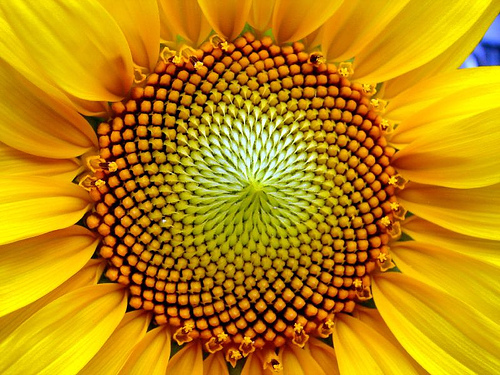
\includegraphics[height=0.25\textheight]{sonnenblume}\quad
    
\includegraphics[height=0.25\textheight]{mandelbrot}\quad
    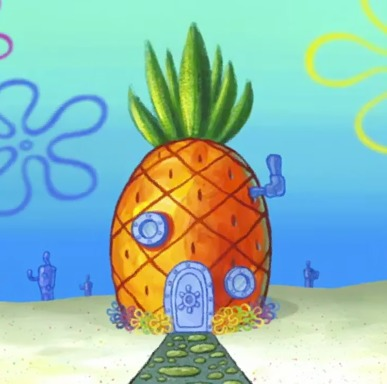
\includegraphics[height=0.25\textheight]{spongebob-ananas}
  \end{center}
}

\begin{frame}\frametitle{Outline}\tableofcontents\end{frame}

% http://joachim-reichel.org/software/fraktal/mandelbrot_large.png


\section{A design pattern in nature}

\begin{frame}\frametitle{A design pattern in nature}
  \begin{center}
    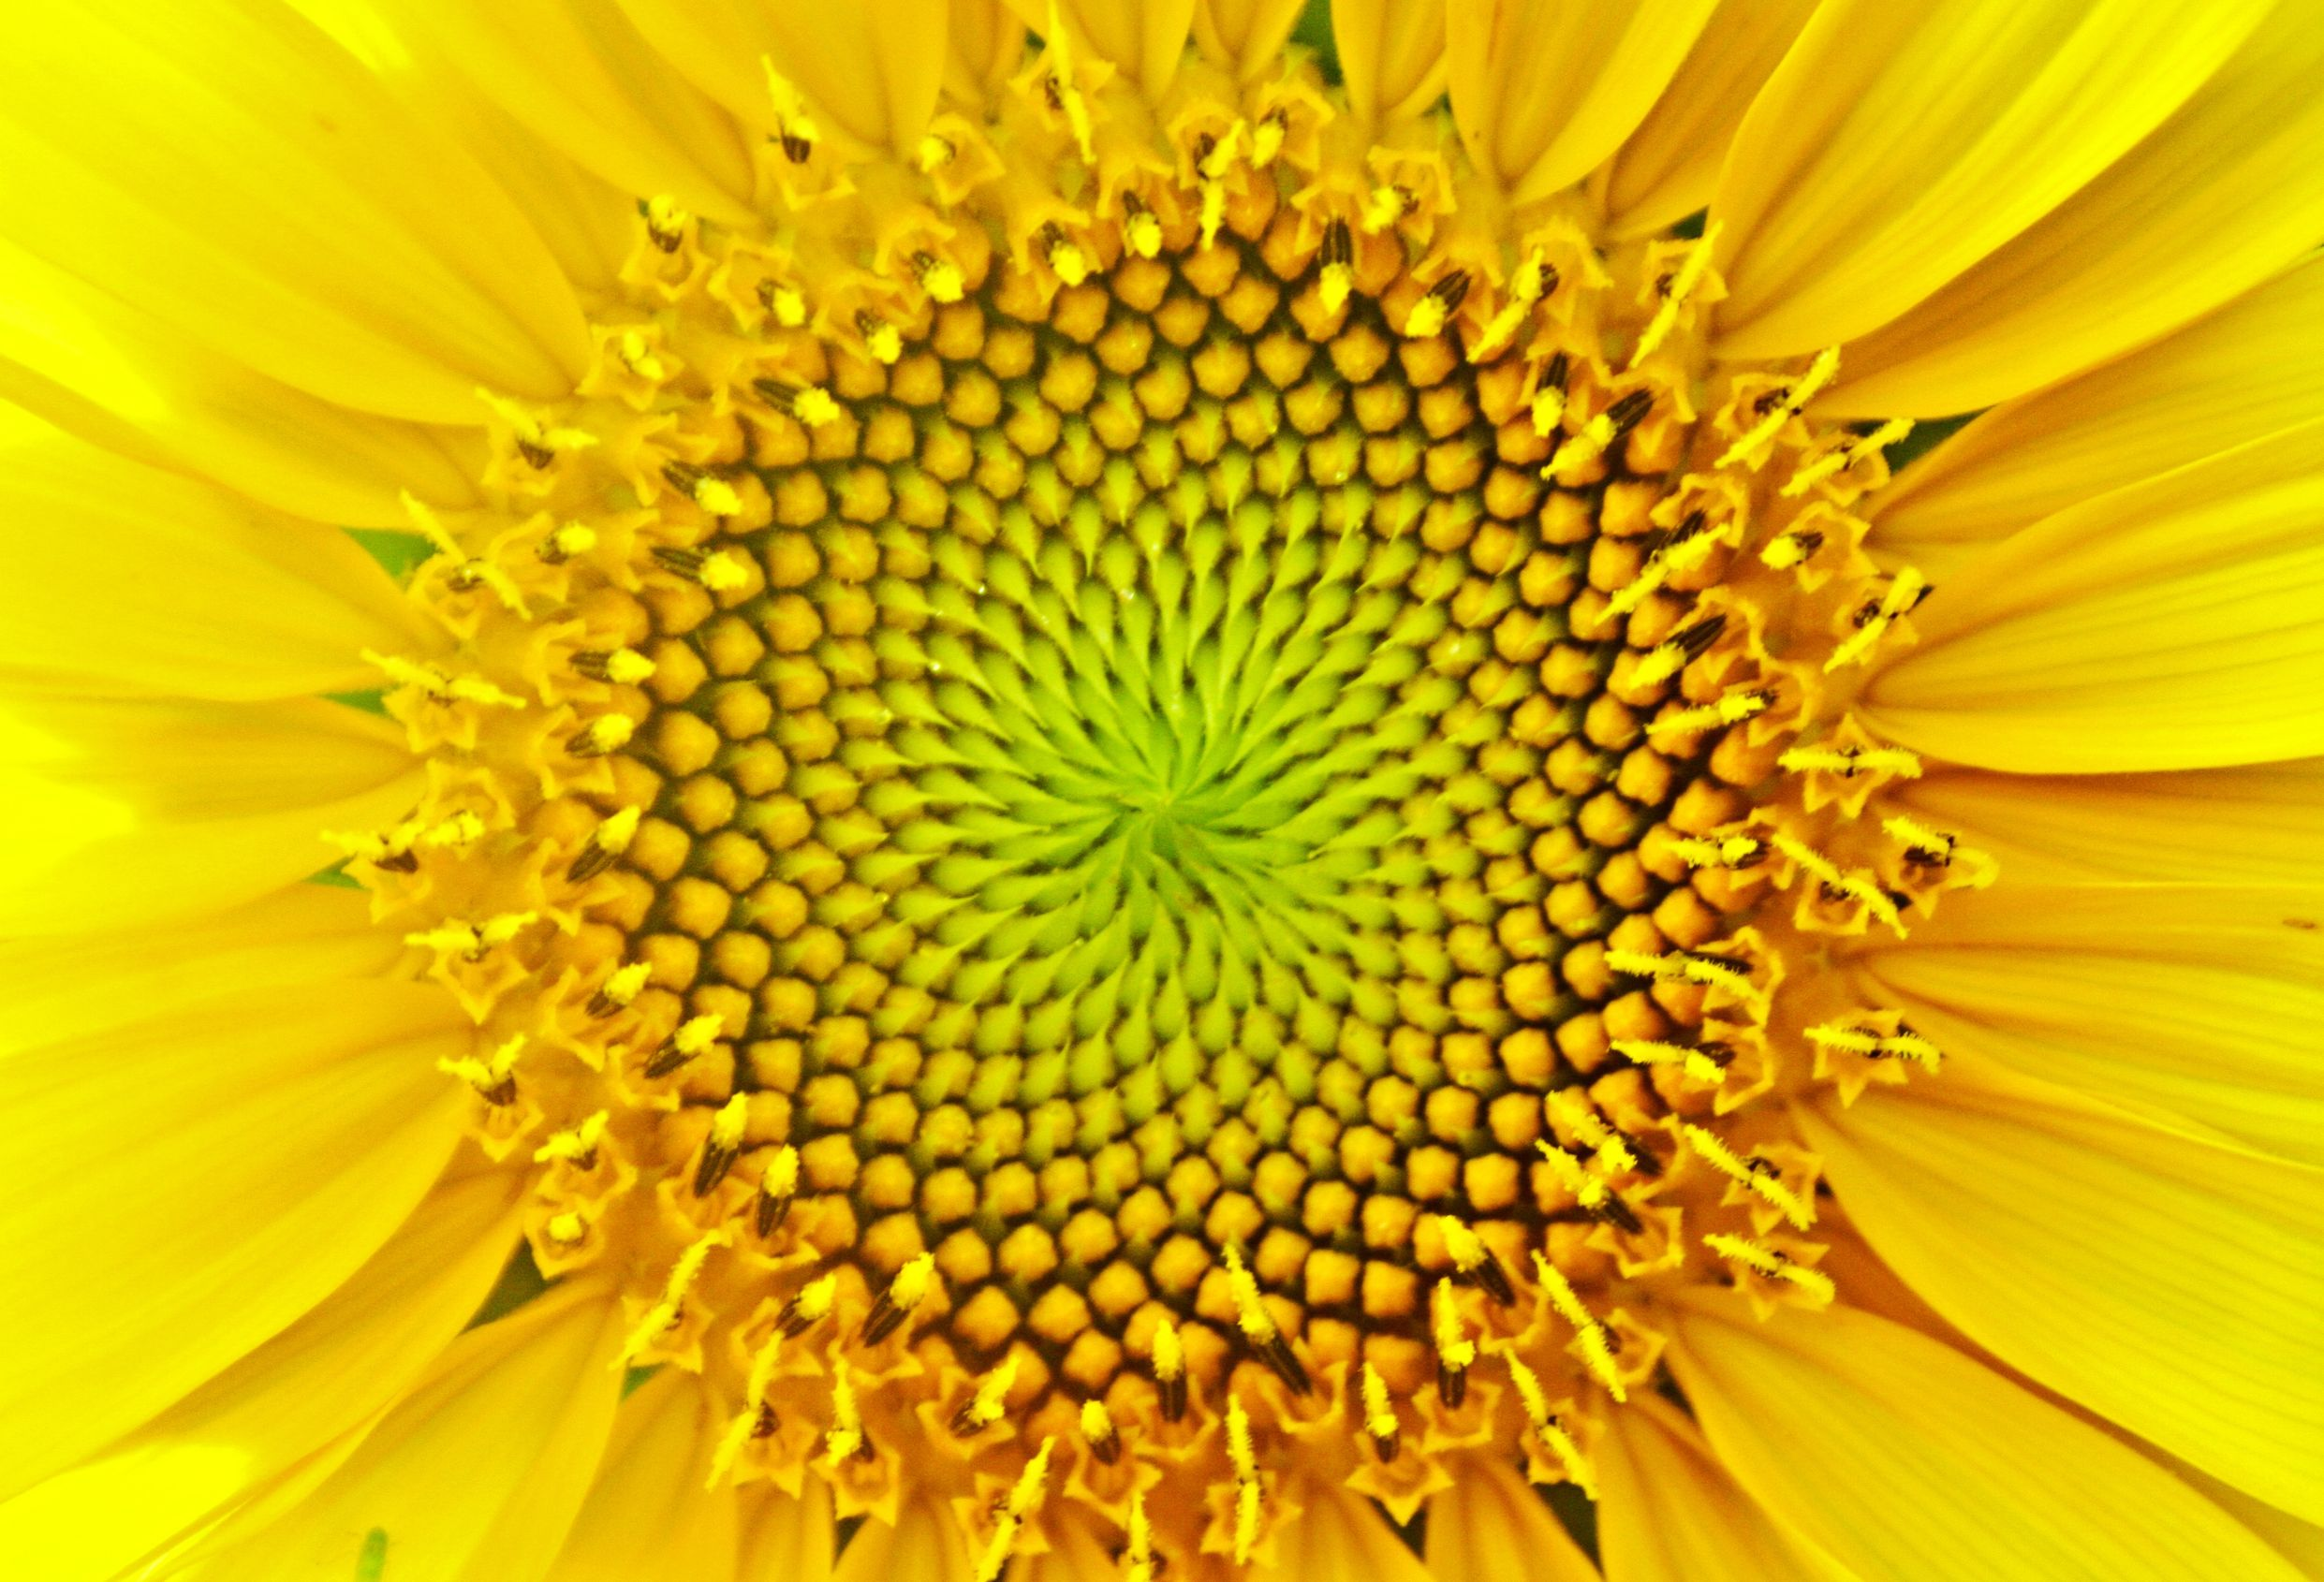
\includegraphics[height=0.6\textheight]{sonnenblume2}
    \bigskip
    % 34 counterclockwise, 21 clockwise

    \only<1>{
      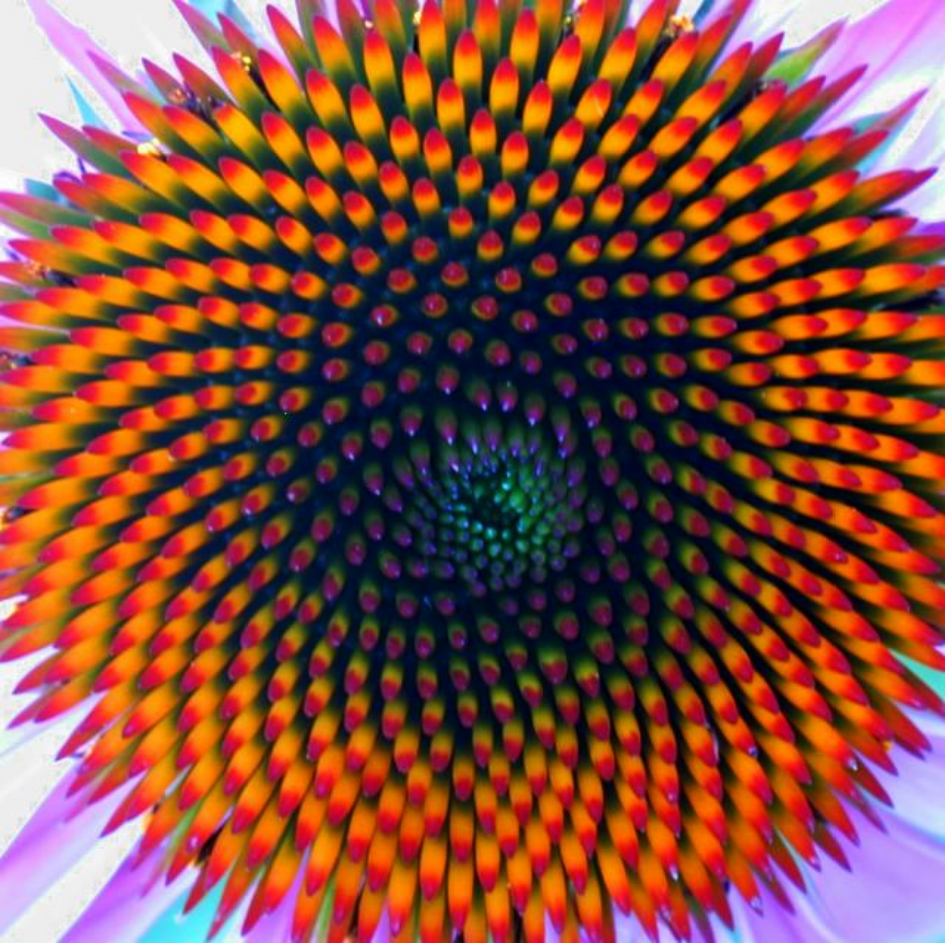
\includegraphics[height=0.2\textheight]{blume}\qquad
      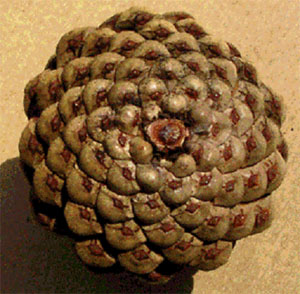
\includegraphics[height=0.2\textheight]{zapfen}\qquad
      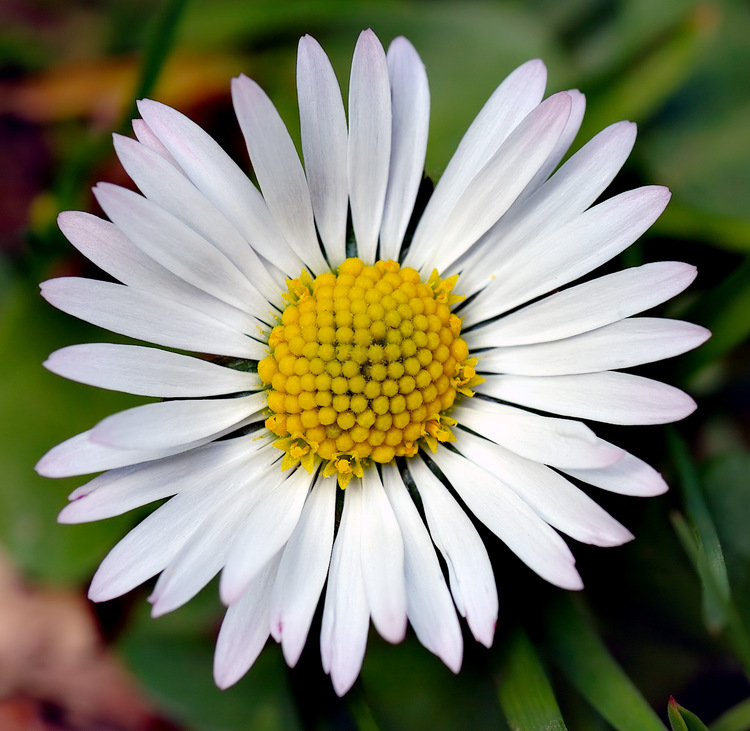
\includegraphics[height=0.2\textheight]{Bellis_perennis_white_(aka)}
    }
    \only<2>{
      \hil{Fibonacci numbers:} \\
      1, 1, 2, 3, 5, 8, 13, 21, 34, 55, \ldots
    }
  \end{center}
\end{frame}


\section{Continued fractions}

\subsection{Examples}

\begin{frame}\frametitle{A curious fraction}
  \only<2-3>{\vspace*{-1em}}
  \only<1>{\Huge}
  \only<1-3>{\[
    \icfrac{1}{2}{2}{2} = {?}
  \]}
  \only<2-3>{\vspace*{1em}}

  \pause
  Crucial observation: Setting
  \only<1-3>{\[ x \defeq {?} - 1 = \icfracc{2}{2}{2}, \]}
  \only<4->{\[ x \defeq {?} - 1 = \icfraccc{2}{2}, \]}
  \pause
  there is the identity
  \[ \frac{1}{2 + x} = x. \]
  \pause
  \pause

  Multiplying by the denominator, we obtain
  \only<5>{$1 = x \cdot (2 + x),$}%
  \only<6->{$1 = 2x + x^2,$}
  \pause
  \pause
  so we only have to solve the quadratic equation
  $0 = x^2 + 2x - 1,$
  \pause
  thus
  \[ x = \frac{-2 + \sqrt{8}}{2} = -1 + \sqrt{2}
    \quad\text{or}\quad
     x = \frac{-2 - \sqrt{8}}{2} = -1 - \sqrt{2}. \]
  It's the positive possibility.
\end{frame}

\begin{frame}\frametitle{More examples}
  \only<1-2>{\vspace*{-2em}\begin{align*}
    \visible<2>{[1; 2, 2, 2, \ldots] =} \icfrac{1}{2}{2}{2} &= \sqrt{2} \\[1.5em]
    \visible<2>{[2; 4, 4, 4, \ldots] =} \icfrac{2}{4}{4}{4} &= \sqrt{5} \\[1.5em]
    \visible<2>{[3; 6, 6, 6, \ldots] =} \icfrac{3}{6}{6}{6} &= \sqrt{10}
  \end{align*}}

  \pause
  \pause

  \begin{enumerate}
    \item $\phantom{0}\sqrt{2} = [1; 2, 2, 2, 2, 2, 2, 2, 2, \ldots]$
    \item $\phantom{0}\sqrt{5} = [2; 4, 4, 4, 4, 4, 4, 4, 4, \ldots]$
    \item $\sqrt{10}           = [3; 6, 6, 6, 6, 6, 6, 6, 6, \ldots]$
    \item $\phantom{0}\sqrt{6} = [2; 2, 4, 2, 4, 2, 4, 2, 4, \ldots]$
    \item $\sqrt{14}           = [3; 1, 2, 1, 6, 1, 2, 1, 6, \ldots]$
    \item $\sbox0{$\sqrt{10}$}\makebox[\wd0][l]{$e$} = [2; 1, 2, 1, 1, 4, 1, 1, 6, \ldots]$
  \end{enumerate}
\end{frame}


\subsection{Calculating the continued fraction expansion}

\begin{frame}\frametitle{The Euclidean algorithm}
  Recall $\sqrt{2} = [1; 2, 2, 2, \ldots] = 1.41421356\ldots$
  \begin{align*}
    1.41421356\ldots &= 1 \cdot 1.00000000\ldots + .41421356\ldots \\
    1.00000000\ldots &= 2 \cdot 0.41421356\ldots + 0.17157287\ldots \\
    0.41421356\ldots &= 2 \cdot 0.17157287\ldots + 0.07106781\ldots \\
    0.17157287\ldots &= 2 \cdot 0.07106781\ldots + 0.02943725\ldots \\
    0.07106781\ldots &= 2 \cdot 0.02943725\ldots + 0.01219330\ldots \\
    0.02943725\ldots &= 2 \cdot 0.01219330\ldots + 0.00505063\ldots \\
    &\,\,\,\vdots
  \end{align*}
\end{frame}

\note{\justifying
  Why does the Euclidean algorithm give the continued fraction coefficients?
  Let's write
  \begin{align*}
    x   &= a_0 \cdot \sbox0{$r_0$}\makebox[\wd0][l]{$1$} + r_0 \\
    1   &= a_1 \cdot r_0 + r_1 \\
    r_0 &= a_2 \cdot r_1 + r_2 \\
    r_1 &= a_3 \cdot r_2 + r_3
  \end{align*}
  and so on, where the numbers~$a_n$ are natural numbers and the residues~$r_n$
  are smaller than the second factor of the respective adjacent product. Then:
  \begin{align*}
    x &= a_0 + r_0 = a_0 + 1/(1/r_0) \\
      &= a_0 + 1/(a_1 + r_1/r_0) = a_0 + 1/(a_1 + 1/(r_0/r_1)) \\
      &= a_0 + 1/(a_1 + 1/(a_2 + r_2/r_1)) = \cdots
  \end{align*}
}

\note{\justifying
  In the beautiful language Haskell, the code for lazily calculating the
  infinite continued fraction expansion is only one line long (the type
  declaration is optional).
  \medskip

  {\scriptsize\texttt{cf :: Double -> [Integer]}\\
  \texttt{cf x = a : cf (1 / (x - fromIntegral a)) where a = floor x}\par}
  \medskip

  So the continued fraction expansion of a number~$x$ begins
  with~$a$, the integral part of~$x$, and continues with the
  continued fraction expansion of~$1 / (x-a)$.
  \medskip

  Note that because of floating-point inaccuracies, only the first few terms of
  the expansion are reliable. For instance,~\texttt{cf (sqrt 6)} could yield
  \texttt{[2,2,4,2,4,2,4,2,4,2,4,2,4,2,4,2,2,1,48,2,4,6,1,\ldots]}.
}


\subsection{Best approximations using continued fractions}

\begin{frame}\frametitle{Best approximations using continued fractions}
  \begin{theorem}
  Cutting off the infinite fraction expansion of a number~$x$
  yields a fraction $a/b$ which is closest to~$x$ under all fractions with
  denominator~$\leq b$.
  \end{theorem}
  \[
    \sqrt{2} = \icfrac{1}{2}{2}{2} \longsquiggly
    1 + \dfrac{1}{2 + \dfrac{1}{2 + \dfrac{1}{2}}} = \frac{17}{12} \approx 1.42
  \]
  \medskip
  \pause

  \hil{Bonus.} The bigger the coefficient after the cut-off is, the better
  is the approximation~$a/b$.
\end{frame}

\note{\justifying
  More precisely, the bonus statement is that the distance from~$x$ to~$a/b$ is
  less than~$1 / (a_n a_{n+1})$, where~$a_n$ is the last coefficient to be
  included in the cut-off and~$a_{n+1}$ is the first coefficient after the
  cut-off.
  \par
}


\section{\texorpdfstring{Approximations of $\pi$}{Approximations of π}}

\begin{frame}[plain,c]
  \centering\Huge
  \scalebox{2.8}{\hil{Love is}}
  \scalebox{2.8}{\hil{important.}}

  \bigskip
  \bigskip

  \scalebox{2.8}{\hil{$\boldsymbol{\heartsuit}$}}
  \par
\end{frame}

\begin{frame}[plain,c]
  \centering\Huge
  \scalebox{2.8}{\hil{Pi is}}
  \scalebox{2.8}{\hil{important.}}

  \bigskip
  \bigskip

  \scalebox{2.8}{\hil{$\boldsymbol{\pi}$}}
  \par
\end{frame}

\begin{frame}\frametitle{Approximations of $\pi$}
  \[ \pi = 3.1415926535\ldots = \icfracccc{3}{7}{15}{1}{292} \]

  \begin{enumerate}
    \item $3$
    \item $[3;7]\phantom{,15,1} = \phantom{0}22/7\phantom{00} = \underline{3.14}28571428\ldots$
    \item $[3;7,15]\phantom{,1} = 333/106 = \underline{3.1415}094339\ldots$
    \item $[3;7,15,1] = 355/113 = \underline{3.141592}9203\ldots$ (Milü)
  \end{enumerate}
\end{frame}


\section{The Mandelbrot fractal}

\begin{frame}\frametitle{The Mandelbrot fractal}
  \centering
  
\includegraphics[width=0.8\textwidth]{mandelbrot}
  \medskip
  \pause

  The Fibonacci numbers show up in the Mandelbrot fractal.
  \par
\end{frame}

\note{\justifying
  See \url{http://math.bu.edu/DYSYS/FRACGEOM2/node7.html} for an explanation of
  why the Fibonacci numbers show up in the Mandelbrot fractal.\par
}


\section{Spirals in nature}

\begin{frame}\frametitle{Spirals in nature}
  \centering
  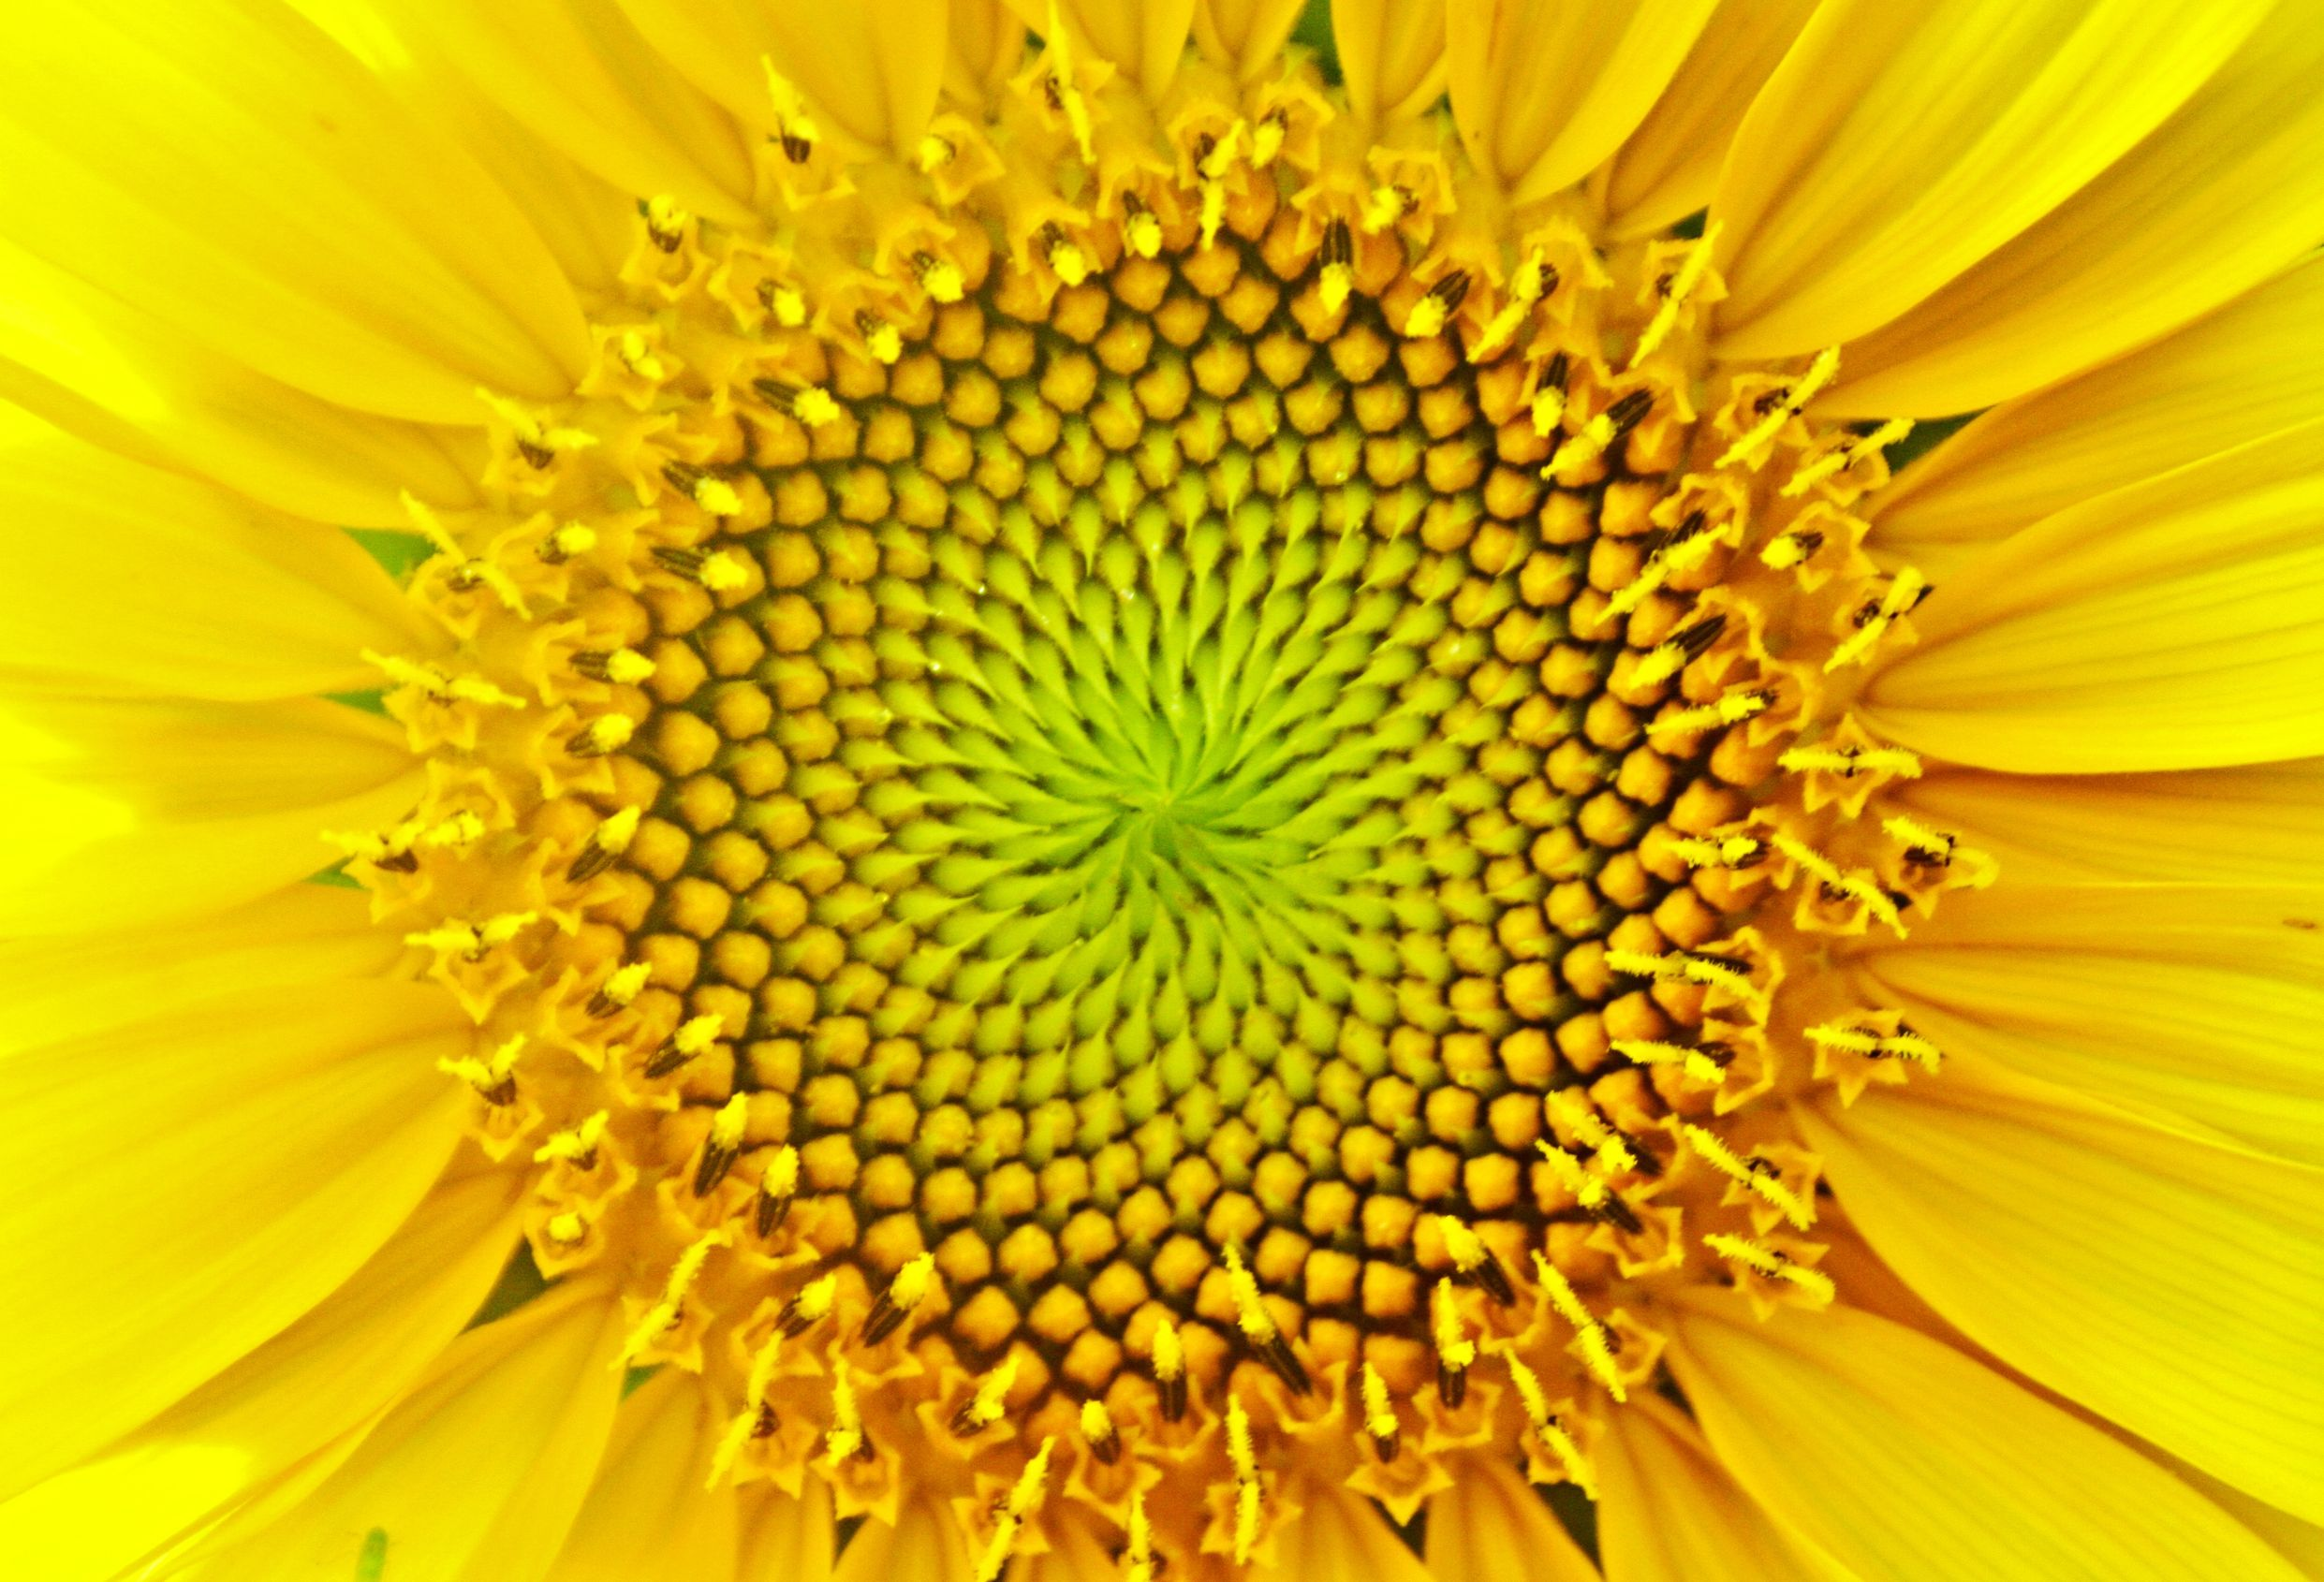
\includegraphics[height=0.8\textheight]{sonnenblume2}
  \par
\end{frame}

\note{\centering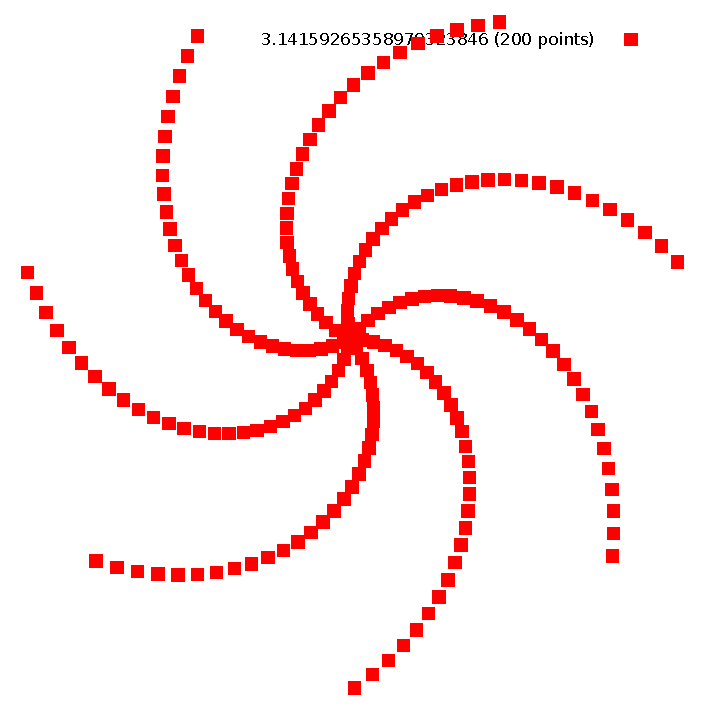
\includegraphics[height=0.95\textheight]{drehwinkel-200-3_14159265358979323846.pdf}\par}
\note{\centering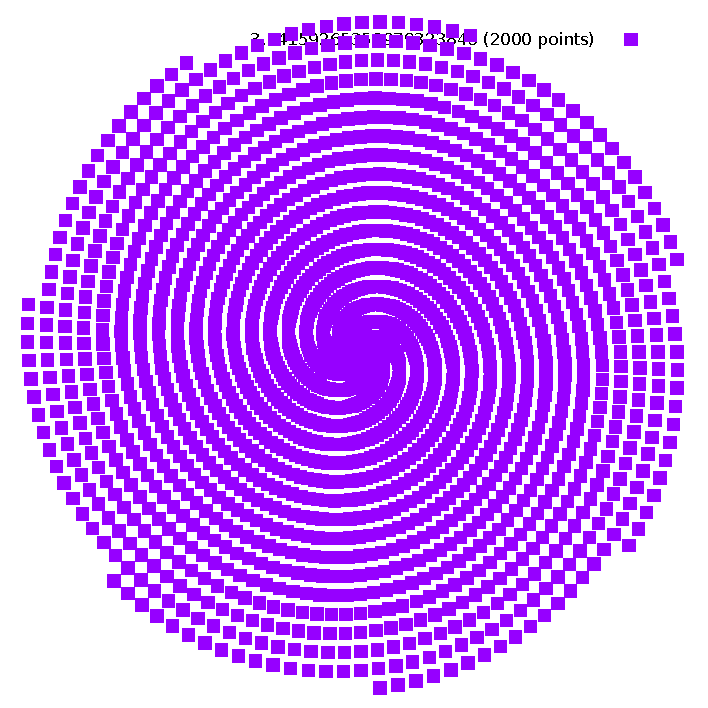
\includegraphics[height=0.95\textheight]{drehwinkel-2000-3_14159265358979323846.pdf}\par}
\note{\centering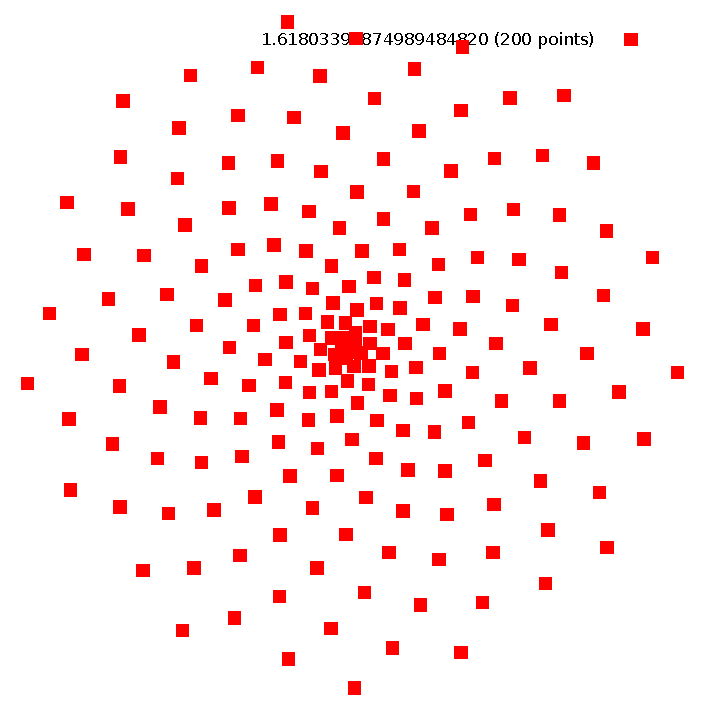
\includegraphics[height=0.95\textheight]{drehwinkel-200-1_61803398874989484820.pdf}\par}
\note{\centering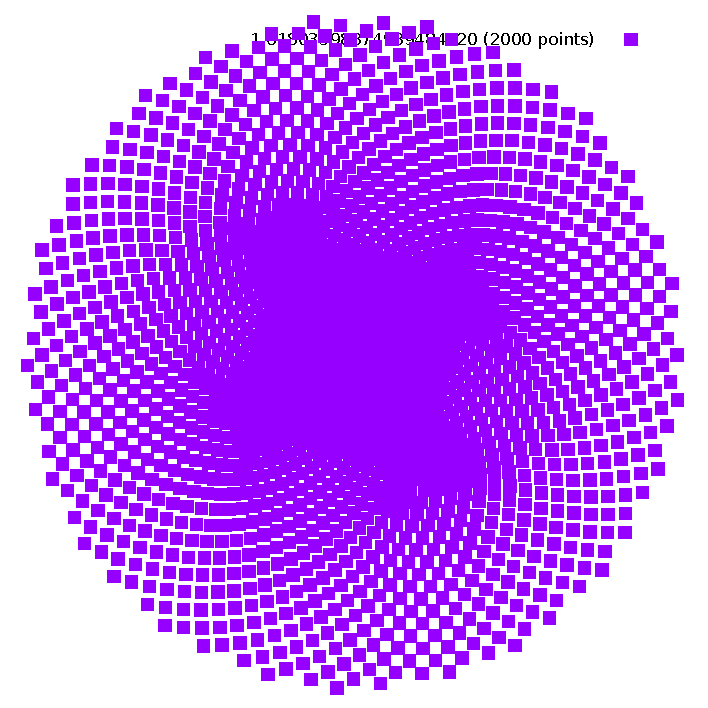
\includegraphics[height=0.95\textheight]{drehwinkel-2000-1_61803398874989484820.pdf}\par}

\begin{frame}\frametitle{The most irrational number}
  For plants, the optimal angle is not \ldots
  \begin{itemize}
  \item $90^\circ = \frac{1}{4} \cdot 360^\circ$ nor is it
  \item $45^\circ = \frac{1}{8} \cdot 360^\circ$.
  \end{itemize}
  Rather, it is the \hil{golden angle} $\Phi \cdot 360^\circ =
  582^\circ$ (equivalently $222^\circ$), where~$\Phi$ is the \hil{golden
  ratio}:
  $\Phi = \frac{1 + \sqrt{5}}{2}$.

  \begin{center}
    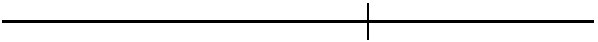
\includegraphics[width=0.7\textwidth]{golden-ratio}
  \end{center}

  \begin{theorem}The golden ratio~$\Phi$ is the \hil{most irrational
  number}.\end{theorem}
  \medskip
  \textbf{Proof.} $\Phi = \icfrac{1}{1}{1}{1}.$
\end{frame}

\begin{frame}\frametitle{Why the Fibonacci numbers?}
  \vspace*{-1em}
  \[ \Phi = \icfrac{1}{1}{1}{1} \]

  \begin{enumerate}
    \item $1\phantom{[,1,1,1,1,1,1,1,1]} = \phantom{0}1/1$
    \item $[1;1]\phantom{,1,1,1,1,1,1,1} = \phantom{0}2/1$
    \item $[1;1,1]\phantom{,1,1,1,1,1,1} \pause = \phantom{0}3/2$
    \item $[1;1,1,1]\phantom{,1,1,1,1,1} \pause = \phantom{0}5/3$
    \item $[1;1,1,1,1]\phantom{,1,1,1,1} \pause = \phantom{0}8/5$ \pause
    \item $[1;1,1,1,1,1]\phantom{,1,1,1} = 13/8$
    \item $[1;1,1,1,1,1,1]\phantom{,1,1} = 21/13$
    \item $[1;1,1,1,1,1,1,1]\phantom{,1} = 34/21$
    \item $[1;1,1,1,1,1,1,1,1] = 55/34$
  \end{enumerate}
\end{frame}


\section{The ananas from SpongeBob SquarePants}

\begin{frame}\frametitle{The ananas from SpongeBob SquarePants}
  \centering
  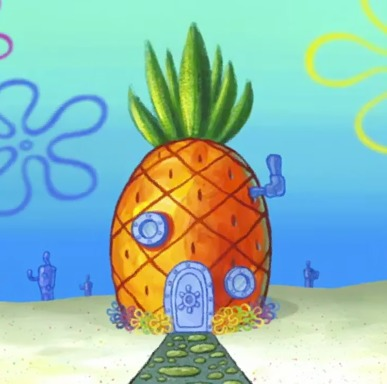
\includegraphics[width=0.65\textwidth]{spongebob-ananas}
  \medskip

  By Vi Hart, recreational mathemusician.
  \par
\end{frame}


\end{document}

Plan of the talk:

1. Images of spirals in nature; notice Fibonacci numbers.
2. Infinite continued fraction:
   * Example with [1; 2, ...]
   * More examples (only listed)
   * Euclidean algorithm (with illustration?)
   * Theorem about best approximation
3. Approximation of pi
   * List original sources for 22/7 and 355/113
   * Explain using continued fractions
4. Spirals in nature
   * angle, need "most irrational number"
   * golden ratio (also explain as a ratio)
   * simulations
5. Fibonacci numbers in the Mandelbrot fractal
6. Vi Hart

Mention rational tangles?

Relation to the number 5.

Translate exercise sheet!
